%Paquetes de latex
\documentclass[journal]{IEEEtran}
\usepackage[spanish,english]{babel}
\usepackage{graphicx}
\usepackage{listings}
\usepackage[utf8]{inputenc}
\usepackage{xcolor}
\usepackage{float}
\usepackage{hyperref}
% Colores para resaltar codigo
\definecolor{codegreen}{rgb}{0,0.6,0}
\definecolor{codegray}{rgb}{0.5,0.5,0.5}
\definecolor{codepurple}{rgb}{0.58,0,0.82}
\definecolor{backcolour}{rgb}{0.95,0.95,0.92}

\lstdefinestyle{mystyle}{
    backgroundcolor=\color{backcolour},   
    commentstyle=\color{codegreen},
    keywordstyle=\color{magenta},
    numberstyle=\tiny\color{codegray},
    stringstyle=\color{codepurple},
    basicstyle=\ttfamily\footnotesize,
    breakatwhitespace=false,         
    breaklines=true,                 
    captionpos=b,                    
    keepspaces=true,                 
    numbers=left,                    
    numbersep=5pt,                  
    showspaces=false,                
    showstringspaces=false,
    showtabs=false,                  
    tabsize=2,
}
\lstset{style=mystyle}
\renewcommand{\lstlistingname}{Código}
\renewcommand\spanishtablename{Tabla}
\graphicspath{ {images/} }

\ifCLASSINFOpdf

\else

\fi



\begin{document}

\title{Manual para generar documentación}

\author{Vicente Romero Andrade}

\markboth{Unidad de Servicios de Cómputo Administrativo, Marzo~2021}
{Shell \MakeLowercase{\textit{et al.}}: }

\maketitle

\selectlanguage{spanish}
% Este es el que escribira el indice
\tableofcontents
%Aqui incia el resumen
\begin{abstract}
En este manual se recopila la metodologia para poder genera documentación de calidad.
Esta documentacion estara en 2 columnas.
\end{abstract}

\IEEEpeerreviewmaketitle

\selectlanguage{spanish}

\IEEEPARstart{E}{ste} es el formato básico para una 
introducción para documentacion en 2 columnas de latex.\\otro párrafo

\section{Instalación}
\subsection{Windows}
Se tienen que instalar los siguientes paquetes.
\begin{itemize}
    \item MikTex, se descarga de aqui \url{https://miktex.org/}
    \item Instalar \href{https://www.activestate.com/products/perl/downloads/}{Perl}
    \item Visual Studio Code, se descarga de aqui \url{https://code.visualstudio.com/}
    \begin{itemize}
        \item Dentro de VS Code instalar la extensión, \href{https://marketplace.visualstudio.com/items?itemName=James-Yu.latex-workshop}{LaTex workshop}
    \end{itemize}
    \item esta \href{https://github.com/ValdrST/Plantilla-LaTeX}{Plantilla} de referencia.
\end{itemize}

\section{Procedimiento}
Soy un texto plano normal que va a generar un parrafo. 
\textbf{Soy un texto en negritas}
\\ 
\textit{Soy un texto en cursiva} y estoy en otro parrafo. \underline{Soy un texto subrayado}
\underline{\textit{\textbf{Soy un texto en cursiva, negritas y subrayado}}}  

\subsection{Soy una subseccion para describir las listas}
\subsubsection{soy una subsubseccion para las listas no ordenadas}
\begin{itemize}
    \item Soy el elemento 1 de una lista
    \begin{itemize}
        \item Soy el elemento 1 de una lista anidada
        \item Soy el elemento 2 de una lista anidada
    \end{itemize}
    \item Soy el elemento 2 de una lista
\end{itemize}

\subsubsection{soy una subsubseccion para las listas ordenadas}
Aqui se describiran las listas orednadas
\begin{enumerate}
    \item soy el elemento 1 de una lista ordenada
    \begin{enumerate}
        \item soy el elemento 1 de una lista ordenada anidada
        \item soy el elemento 2 de una lista ordenada anidada
    \end{enumerate}
    \item soy el elemento 2 de una lista ordenada
    \item soy el elemento 3 de una lista ordenada
\end{enumerate}
\subsection{Soy una subseccion que describira como citar codigo}
\subsubsection{Traer codigo fuente externo}
El codigo fuente puede venir de un archivo
\lstinputlisting[language=Python,caption=Ejemplo python,label={lst:codigo_python}]{codigo_fuente_python.py}
\subsubsection{Traer codigo fuente en el mismo documento}
o puede escribirse en el mismo documento
\begin{lstlisting}[language=bash, caption=Bomba fork,label={lst:bomba_fork}]
#!/bin/bash
bomba(){
  bomba | bomba & 
}
bomba
\end{lstlisting}

\subsection{Soy una subseccion que describira como traer imagenes}
Para esta seccion se pueden traer imagenes
\subsubsection{Imagen de ruta relativa}
Esta imagen esta con ruta relativa y texto
\begin{figure}[H]
    \centering
    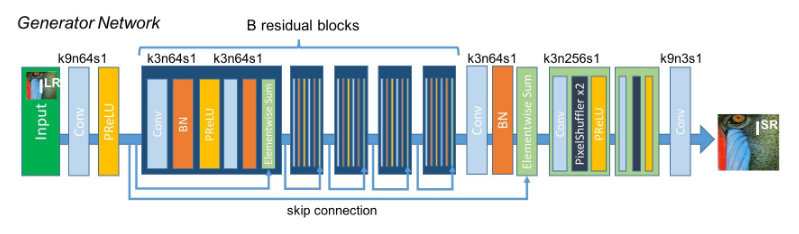
\includegraphics[scale=.20]{images/Generador.png}
     \caption{Imagen de ruta relativa con texto}
     \label{fig:SRGANGEN}
 \end{figure}
 \subsubsection{Imagen simple sin texto}
Esta imagen no lleva texto por lo que no se indexa en tabla de figuras
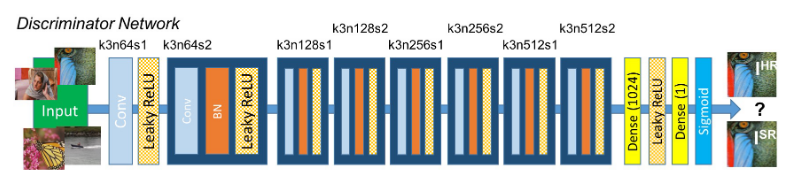
\includegraphics[scale=.28]{images/Discriminador.png}

\subsection{Tablas}
\subsubsection{Tablas con texto indexables}
Estas tablas se pueden indexar sin problemas
\begin{table}[h!]
    \centering
    \begin{tabular}{||c c c c||} 
     \hline
     Col1 & Col2 & Col2 & Col3 \\ [0.5ex] 
     \hline
     1 & 6 & 87837 & 787 \\ 
     2 & 7 & 78 & 5415 \\
     3 & 545 & 778 & 7507 \\
     4 & 545 & 18744 & 7560 \\
     5 & 88 & 788 & 6344 \\ [1ex] 
     \hline
    \end{tabular}
    \caption{Tabla con texto indexable y citable}
    \label{tabla:1}
    \end{table}
\subsubsection{Tablas simples}
estas tablas son la forma simple, se pueden acomodar al texto,
o al parrafo dado segun se acomoden y segun la longitud del texto.

\begin{tabular}{||c c||} 
    \hline
    Col1 & Col2 \\ [0.5ex] 
    \hline
    1 & 6  \\ 
    2 & 7 \\
    3 & 545 \\
    4 & 545 \\
    5 & 88  \\ [1ex] 
    \hline
\end{tabular}
\\
\subsection{Citar elementos}
Si se requiere citar tablas, figuras o referencias esta es la seccion
\subsubsection{Referencias}
Las referencias tienen un nombre y se ven asi \cite{ledig} o asi \cite[Trabajo de ledig]{ledig}
\subsubsection{Figuras o imagenes}
Tambien se puede referenciar a un a una figura \ref{fig:SRGANGEN}
\subsubsection{Codigo}
Se puede citar codigo \ref{lst:bomba_fork}
\subsubsection{Tablas}
Se pueden referenciar tablas, como en la tabla \ref{tabla:1}
%% Forzar nueva pagina \newpage

\newpage
\listoffigures
\listoftables
\lstlistoflistings

\begin{thebibliography}{2}

\bibitem{ledig}
Christian Ledig, Lucas Theis, Ferenc Huszár, José Antonio Caballero,Andrew Aitken, Alykhan Tejani, Johannes Totz, Zehan Wang, and Wenz-he Shi. Photo-realistic single image super-resolution using a generativeadversarial network.2017 IEEE Conference on Computer Vision andPattern Recognition (CVPR), pages 105–114, 2016.
\bibitem{Dong}
Dong, Hao and Supratak, Akara and Mai, Luo and Liu, Fangde and Oehmichen, Axel and Yu, Simiao and Guo, Yike. TensorLayer: A Versatile Library for Efficient Deep Learning Development.2017 ACM Multimedia, http://tensorlayer.org.
\bibitem{Calcagni}
L.Calcagni.Super    resolution    generative    adver-sarialnetwork.https://github.com/lcalcagni/Super-resolution-Generative-Adversarial-Network, 2020.
\bibitem{PRELU}
Kaiming He, Xiangyu Zhang, Shaoqing Ren, Jian Sun.
Delving Deep into Rectifiers: Surpassing Human-Level Performance on ImageNet Classification. 2015 IEEE International Conference on Computer Vision (ICCV) (2015): 1026-1034.
\bibitem{REDRES}
K. He, X. Zhang, S. Ren, and J. Sun. Deep residual learning for imagerecognition.2016 IEEE Conference on Computer Vision and PatternRecognition (CVPR), pages 770–778, 2016.
\end{thebibliography}

\end{document}


